*** messages surrounded by three * are notes to the reviewer, if you'd like to ctrl-f for them ***

This chapter first presents the atomic fraction of particular isotopes, the reports the results of the three model variation tests.

\section{Fuel Isotopic Compositions}

The isotopic compositions in the Sangamon20 full-core models use those generated from an infinite cubic lattice of pebbles, which use explicitly modeled TRISO particles.  The fuel is fresh at the first depletion time step, and goes through six burnup cycles, each lasting six months.
\begin{figure}[H]
\centering
%
\begin{subfigure}{0.4\textwidth}
  \includegraphics[width=0.95\linewidth]{figures/burn-20-bstep0}
  \caption{Fresh}
  \label{fig:bstep0}
\end{subfigure}%
%
\begin{subfigure}{0.4\textwidth}
  \includegraphics[width=0.95\linewidth]{figures/burn-20-bstep1}
  \caption{Six Months}
  \label{fig:bstep1}
\end{subfigure}%

\caption{Serpent-generated mesh figures of the fission rate (hot color map) and thermal flux (cold color map) for the representative single-pebble at each depletion step.  A cold color map is from shades of whitish-blue (high) to blackish-blue (low) while the hot color map is from a whitish-yellow (high) to reddish-brown (low)}
\end{figure}

\begin{figure}[H]\ContinuedFloat
\centering

\begin{subfigure}{0.4\textwidth}
  \includegraphics[width=0.95\linewidth]{figures/burn-20-bstep2}
  \caption{Twelve Months}
  \label{fig:bstep2}
\end{subfigure}%
%
\begin{subfigure}{0.4\textwidth}
  \includegraphics[width=0.95\linewidth]{figures/burn-20-bstep3}
  \caption{Eighteen Months}
  \label{fig:bstep3}
\end{subfigure}%

\begin{subfigure}{0.4\textwidth}
  \includegraphics[width=0.95\linewidth]{figures/burn-20-bstep4}
  \caption{Twenty-Four Months}
  \label{fig:bstep4}
\end{subfigure}%
%
\begin{subfigure}{0.4\textwidth}
  \includegraphics[width=0.95\linewidth]{figures/burn-20-bstep5}
  \caption{Thirty Months}
  \label{fig:bstep5}
\end{subfigure}%

\begin{subfigure}{0.4\textwidth}
  \includegraphics[width=0.95\linewidth]{figures/burn-20-bstep6}
  \caption{Thirty-Six Months}
  \label{fig:bstep6}
\end{subfigure}%
%
\caption{Serpent-generated mesh figures of the fission rate (hot color map) and thermal flux (cold color map) for the representative single-pebble at each depletion step.  A cold color map is from shades of whitish-blue (high) to blackish-blue (low) while the hot color map is from a whitish-yellow (high) to reddish-brown (low). (cont)}
\label{fig:burn-meshes}
\end{figure}
Figure \ref{fig:burn-meshes} depicts the evolution of the fission rate (hot color map) and thermal flux (cold color map) over the seven stages.  The maximum cutoff for thermal flux is 0.625 eV in these figures.  Over successive depletion steps, the fission rate decreases, and thermal flux increases.
\begin{figure}[H]
\centering
%
\begin{subfigure}{0.95\textwidth}
  \includegraphics[width=0.95\linewidth]{figures/compositions/iodine}
  \caption{Iodine}
  \label{fig:i}
\end{subfigure}%

\begin{subfigure}{0.95\textwidth}
  \includegraphics[width=0.95\linewidth]{figures/compositions/xenon}
  \caption{Xenon}
  \label{fig:xe}
\end{subfigure}%

\caption{Evolution of Certain Isotopic Concentrations in Pebbles over Six Six-Month Passes (cont.)}
\end{figure}

\begin{figure}[H]\ContinuedFloat
\centering

\begin{subfigure}{0.95\textwidth}
  \includegraphics[width=0.95\linewidth]{figures/compositions/caesium}
  \caption{Caesium}
  \label{fig:cs}
\end{subfigure}%


\begin{subfigure}{0.95\textwidth}
  \includegraphics[width=0.95\linewidth]{figures/compositions/radium}
  \caption{Radium}
  \label{fig:ra}
\end{subfigure}%

\caption{Evolution of Certain Isotopic Concentrations in Pebbles over Six Six-Month Passes (cont.)}
\end{figure}

\begin{figure}[H]\ContinuedFloat
\centering


\begin{subfigure}{0.95\textwidth}
  \includegraphics[width=0.95\linewidth]{figures/compositions/thorium}
  \caption{thorium}
  \label{fig:th}
\end{subfigure}%

\begin{subfigure}{0.95\textwidth}
  \includegraphics[width=0.95\linewidth]{figures/compositions/uranium}
  \caption{Uranium}
  \label{fig:u}
\end{subfigure}%

\caption{Evolution of Certain Isotopic Concentrations in Pebbles over Six Six-Month Passes (cont.)}
\end{figure}

\begin{figure}[H]\ContinuedFloat
\centering

\begin{subfigure}{0.95\textwidth}
  \includegraphics[width=0.95\linewidth]{figures/compositions/plutonium}
  \caption{Plutonium}
  \label{fig:pu}
\end{subfigure}%

\caption{Evolution of Certain Isotopic Concentrations in Pebbles over Six Six-Month Passes (cont.)}
\label{fig:comps}
\end{figure}

The full isotopic inventory tracked in the Sangamon20 reactor models extends far beyond those supplied in Figure \ref{fig:comps}.  For a full list, see ***ref zenodo comps*** for the compositions alone, or ***ref phlox zenodo*** for a complete input file and associated output.  Figure \ref{fig:comps} omits any stable isotope, and focuses on those of interest in safety analysis.

The only the xenon content rivals the inventory of uranium.  All isotopes of uranium steadily increase over time with the exception of $^{235}U$, ending at 0.0647 by atomic fraction in the sixth pass.  $^{232}U$, initially the smallest fraction of uranium sees the most dramatic increase over time, increasing by two orders of magnitude between the first ($9.28\times10^{-12}$) and sixth ($1.9\times10^{-10}$) cycle.  While the atomic fraction doesn't reach an equilibrium, the rate at which it increases each cycle is steady by the third pass - increasing by $4.02\times10^{-11}$,$4.2\times10^{-11}$, and $3.9\times10^{-11}$ from the third to fourth, fourth to fifth, and fifth to sixth pass, respectively.  Plutonium content is also fairly high, with $^{239}Pu$ peaking at 0.00439.  However, unlike many other isotopes, which peak in the sixth cycle, $^{239}Pu$ crests in the third and fourth passes, decreasing from 0.00439 in the fourth pass to 0.00380 in the sixth.  Pu-238, meanwhile, is the least abundant, but does experience the most dramatic increase over time (especially between the first and second passes).



$^{133}Xe$ seems to be steady around its initial concentration of $2.86\times10^{-05}$ atomic fraction, decreasing only to $2.68\times10^{-05}$ by the sixth pass.  $^{135}Xe$ decreases a bit more dramatically, going from an initial $9.70\times10^{-07}$ after its first six months, to  $6.46\times10^{-07}$ after thirty-six months.  $^{136}Xe$ is both the greatest contributor to xenon content in the fuel, and the only isotope reported in  Figure \ref{fig:xe} to increase, owing to its long half life.  Each cycle increases $^{136}Xe$ content by ~0.0011, beginning at a concentration of 0.00105 in the first cycle and ending at 0.0066 after the sixth.  Isotopes of iodine form a smaller portion of fission products than xenon or caesium (still a relatively high magnitude) which is of concern due to its high mobility in water and uptake in the thyroid.  $^{129}I$ is the most abundant isotope of iodine reported here.  It increases for the entirety of the pebble's life, beginning at $7.38\times10^{-05}$ and peaking at 0.000538 at its discharge burnup.  $^{130}I$ and $^{135}I$ are both relatively stable, most likely due to their short half-lives, combined with transmutation after undergoing neutron capture.  While $^{130}I$ is the least abundant, it increases over time.  Caesium has a net concentration similar to xenon's.  Unsurprisingly $^{135}Cs$ and $^{137}Cs$, which both have half-lives longer than a pebble's stint in the reactor, are in greatest abundance, and increase over time.

Of the elements reported here, radium and thorium are in lowest abundance.  $^{225}Ra$ only appears in trace amounts (less than or equal to $9.99\times10^{-20}$) for the first three passes.  $^{224}Ra$ far outweighs the other reported isotopes of radium, with an atomic fraction of $7.46\times10^{-15}$ after thirty-six months - two orders of magnitude higher than all other isotopes of radium combined at this depletion step.  Thorium has the second-least abundant atomic fractions, with fertile $^{232}Th$ being the most abundant, at $8.80\times10^{-10}$ in the sixth pass.

\section{Full-Core Control Model}

Figure \ref{fig:control} shows a cross section of the core geometry at the origin in the xy and xz planes (Sub-Figures a and c, respectively) and provides a mesh of the fission rate and thermal flux in the xy and xz planes (Sub-Figures b and d, respectively).  Both of these integrate over z and y, respectively, to produce a 2D image.  Analytically calculated $k_{eff}$ was 1.04077 $\pm$ 0.00054.
\begin{figure}[h!]
\centering
\includegraphics[width=0.6\linewidth]{figures/geom-legend}
\caption{Legend for Geometry Figures}
\label{fig:geom-legend}
\end{figure}

Figure \ref{fig:geom-legend} is accurate for all cross sections of reactor geometry.  In homogenized simulations, the shades of green represent the material blend forming the center of the pebble at a given burnup.  For heterogenized simulations, these same shades represent the TRISO particle kernel at a particular burnup.

\begin{figure}
\centering

\begin{subfigure}{0.45\textwidth}
  \includegraphics[width=0.95\linewidth]{figures/control/control-r}
  \caption{Radial Cross Section at y=0}
  \label{fig:bstep0}
\end{subfigure}%
%
\begin{subfigure}{0.45\textwidth}
  \includegraphics[width=0.95\linewidth]{figures/control/control-rm}
  \caption{Radial Mesh}
  \label{fig:bstep1}
\end{subfigure}

\begin{subfigure}{0.45\textwidth}
  \includegraphics[width=0.95\linewidth]{figures/control/control-v}
  \caption{Axial Cross Section at z=0 }
  \label{fig:bstep1}
\end{subfigure}
%
\begin{subfigure}{0.45\textwidth}
  \includegraphics[width=0.95\linewidth]{figures/control/control-vm}
  \caption{Axial Mesh}
  \label{fig:bstep1}
\end{subfigure}
%
\caption{Full Core}
\label{fig:control}
\end{figure}


The mesh in Figure \ref{fig:controlb} shows bands of concentric rings around the outer edges of the active core.  These bands suggest that the outermost areas of the core are regions of high fission activity relative to the center, which is at odds with what most might expect from the neutronics behavior in a cylindrical reactor.  Certainly the pebbles are physically forming rings at the outer edges, and their placement becomes more haphazard toward the center.  However, the high intensities seen in this outer region in the mesh figures are unindicative of a total flux profile showing the same.  Remember that Serpent 2 integrates over the z direction to produce a 2D plot of the xy plane.  For a cylinder, the distance in z each point integrates over is the same - the height of the reactor.  However, points at the outermost regions are integrating in a volume composed more of pebbles - and therefore fissile material - than the center, where more space filled with coolant.

In Figure \ref{fig:controld} we can see a similar banding effect on the top and bottom edge of the core region, but not on the sides.  No hot-spots on the edges because Figure \ref{fig:controld} is in the xz plane, and integrates over y.  However, for a cylinder, the distance integrated over is not the same at all points.  At the centerline, the distance is simply the diameter.  However, as you move towards the edge, the distance integrated over approaches zero.

\begin{figure}[H]
\centering

\begin{subfigure}{0.9\textwidth}
  \includegraphics[width=0.95\linewidth]{figures/therm_flux_homog.png}
  \caption{Thermal Flux}
  \label{fig:hom-det-xy-therm}
\end{subfigure}%

\caption{Radial Thermal and Fast Flux Profiles}
\end{figure}

\begin{figure}[H]\ContinuedFloat
\centering

\begin{subfigure}{0.9\textwidth}
  \includegraphics[width=0.95\linewidth]{figures/fast_flux_homog.png}
  \caption{Fast Flux}
  \label{fig:hom-det-xy-fast}
\end{subfigure}

%
\caption{Radial Thermal and Fast Flux Profiles (cont.)}
\label{fig:hom-det-xy}
\end{figure}
\begin{figure}[h!]
\centering

\begin{subfigure}{0.6\textwidth}
  \includegraphics[width=0.95\linewidth]{figures/therm_flux_homog_z.png}
  \caption{Thermal Flux}
  \label{fig:hom-det-z-therm}
\end{subfigure}%
%
\begin{subfigure}{0.6\textwidth}
  \includegraphics[width=0.95\linewidth]{figures/fast_flux_homog_z.png}
  \caption{Fast Flux}
  \label{fig:hom-det-z-fast}
\end{subfigure}

%
\caption{Axial Thermal and Fast Flux Profiles}
\label{fig:hom-det-z}
\end{figure}

***I know that there should be continuity at 0 between the axial and radial flux profiles, and there currently is a difference of 3 orders of magnitude.  I believe this is because of differing bin sizes between the detector that tracked the axial fluxes, and the detector that tracked the fluxes at the xy plane.  Basically, in the axial detector, each bin had a defined length in z, 0.1 cm or what-have-you.  However, these bins had no x or y limitations, and covered all x and y at that point (the bins are shaped like a stack of pancakes or such).  For the radial detector, I had to create the detector bins such that they formed a uniform grid over the xy plane, centered on the origin (which is the physical center of the reactor).  These bins were finite in x and y, but not in the z direction, so they covered all z that fell within the limits of the bin (these bins are like a long rectangular prism).  While this uniform grid prevents the radial flux profile from warping, which is what happens if you attempt to make a detector along only one axis (the bins end up being unequal sizes), the fact that the axial detector bins differ from the radial detector bins means they don't match each other.

tl;dr: should I divide the neutron flux by bin volume so the axial and radial profiles match in magnitude (hopefully)***

Figures \ref{fig:hom-det-xy} and \ref{fig:hom-det-z} provide the fast and thermal flux profiles in Sangamon20.  The former are the radial fluxes, along the x-axis, and the latter are the center line profiles.  Both axially and radially, the thermal flux sees a 'bump', which peaks approximately 10 cm into the reflector, at 100 cm.  These are the highest peaks in the thermal flux, with the second highest thermal flux being at the center line.  For the fast flux profile we see a flattened peak in the  active core (-90.0 cm to 90 cm) and 10 cm into the reflector.  Fast flux rapidly decreases in the reflector as fast neutrons down scatter in the graphite.

Both Figures \ref{fig:hom-det-xy} and \ref{fig:hom-det-z} show that while the radial banding seen in the fission rate mesh profiles are of high intensity, the flux peaks are elsewhere.


\begin{figure}[h!]
\centering

\begin{subfigure}{0.6\textwidth}
  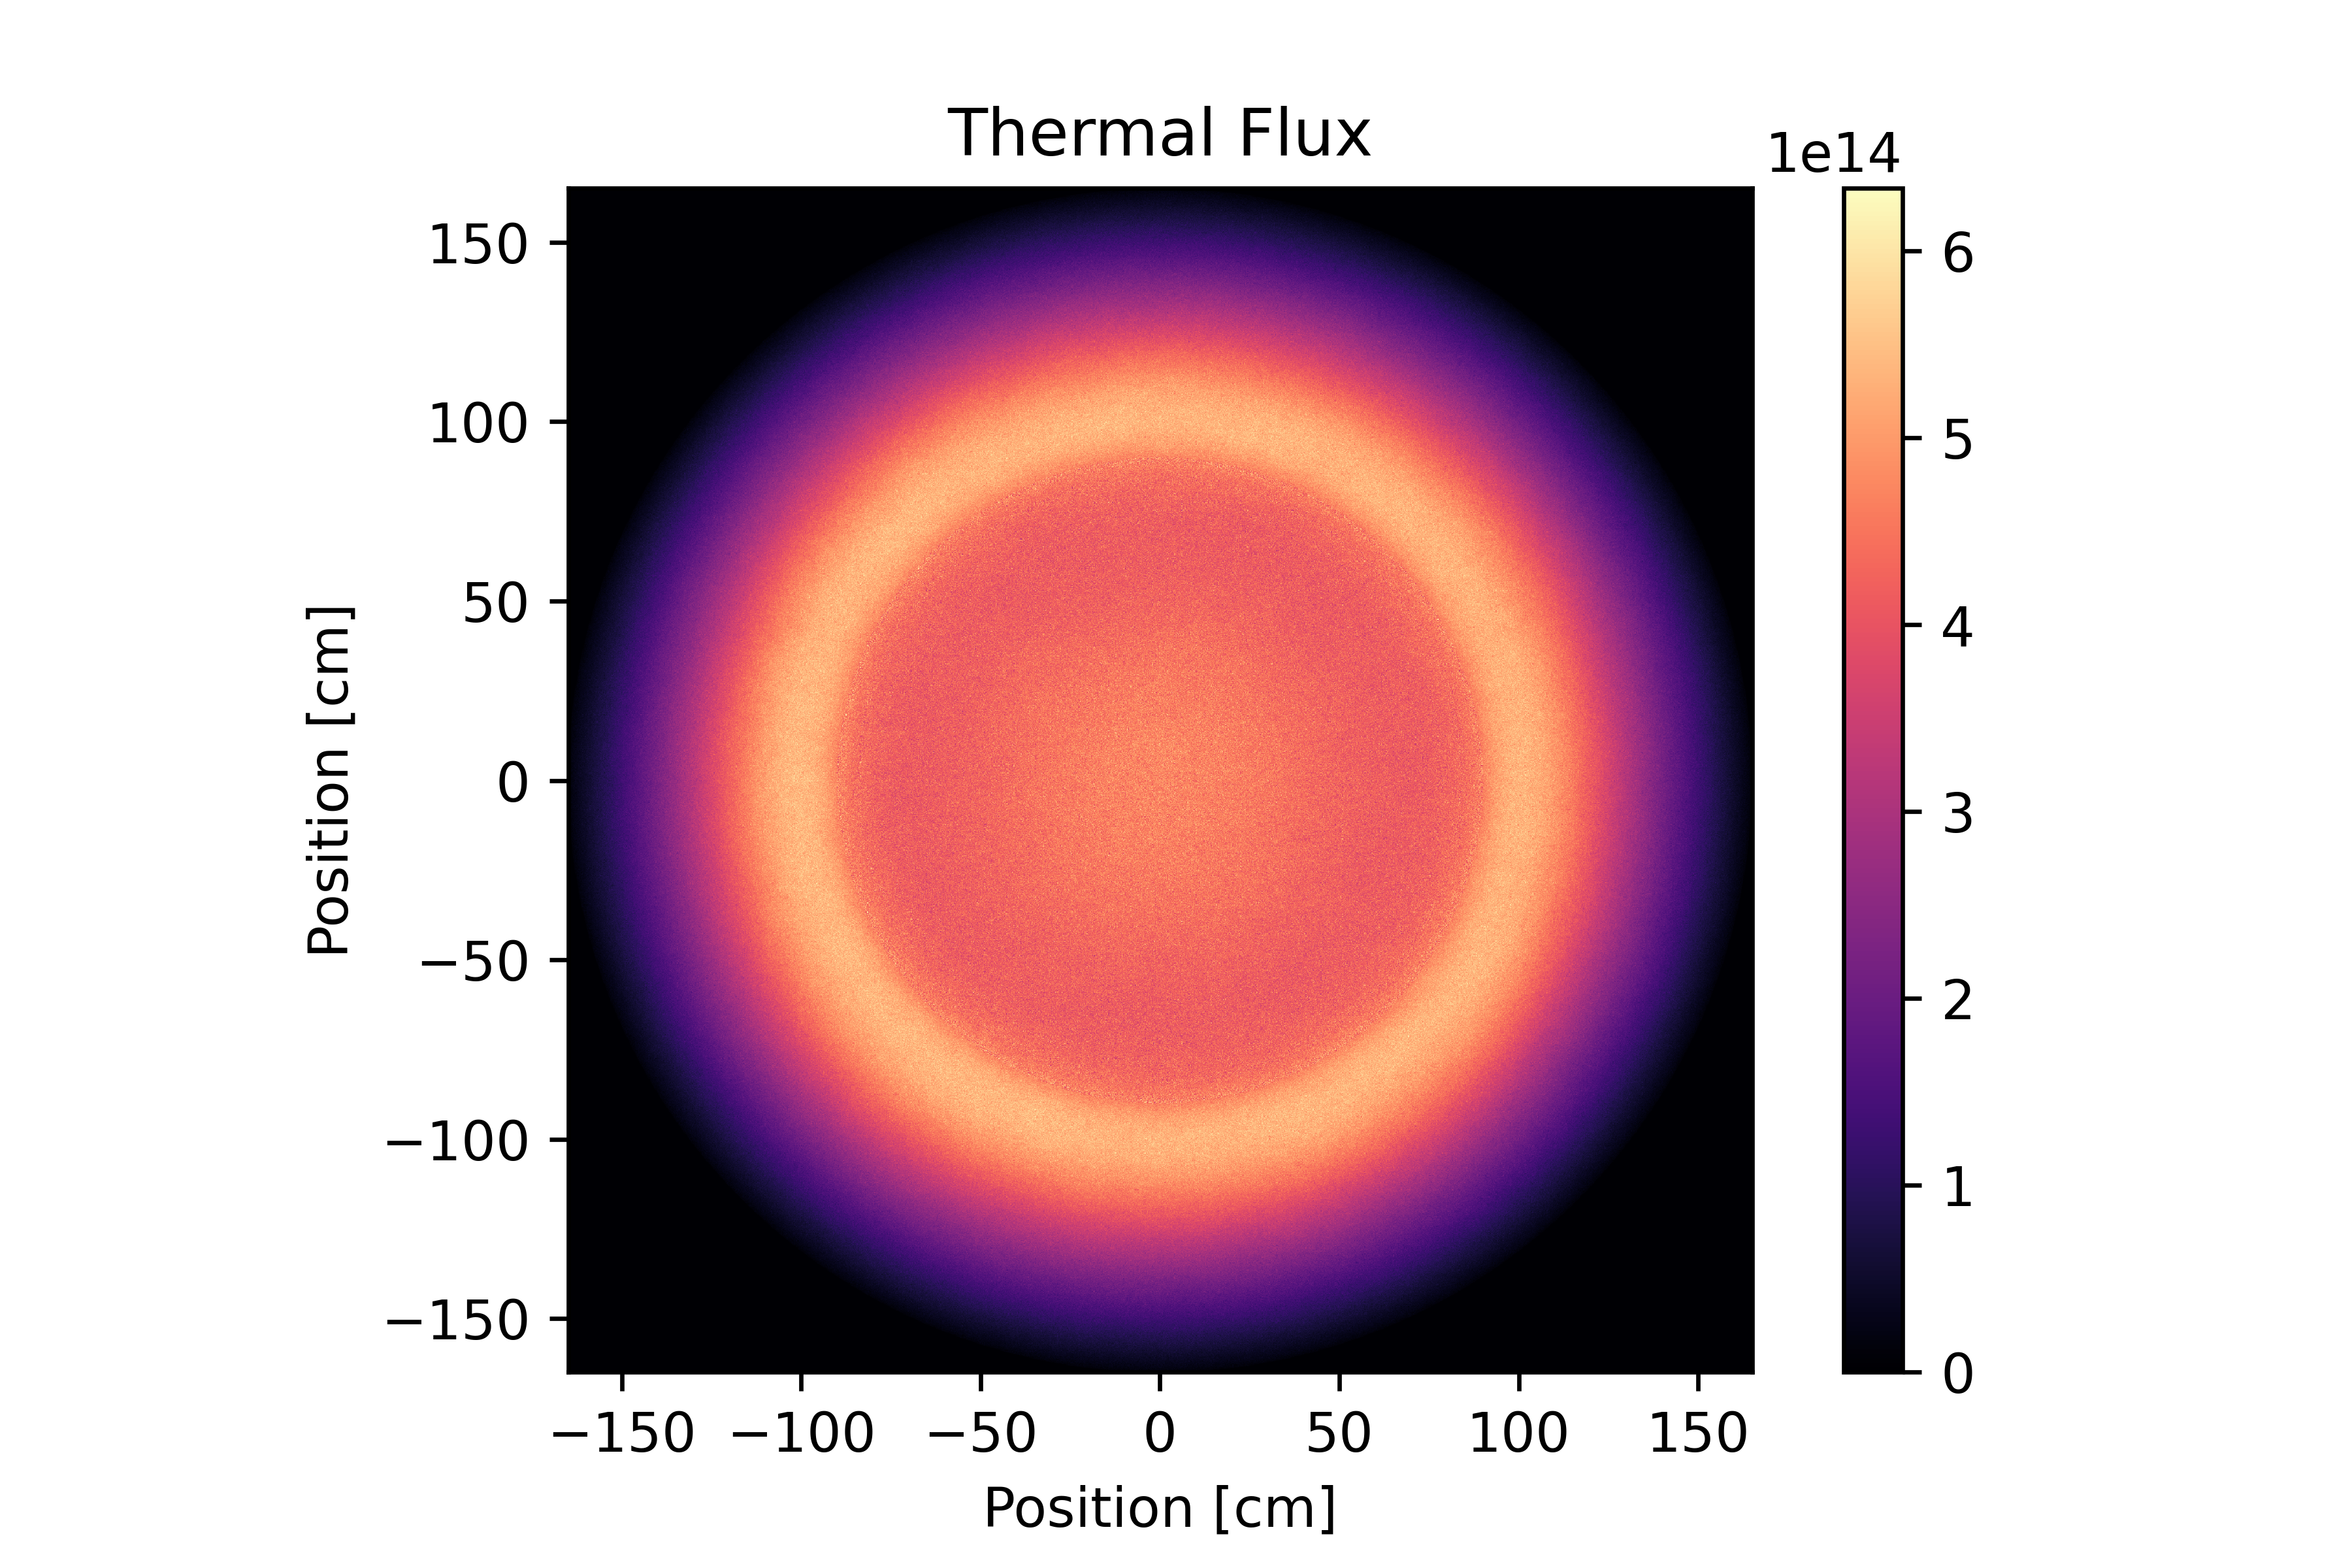
\includegraphics[width=0.95\linewidth]{figures/therm_xy_plane_homog.png}
  \caption{Thermal Flux in xy Plane}
  \label{fig:hom-plane-therm}
\end{subfigure}%
%
\begin{subfigure}{0.6\textwidth}
  \includegraphics[width=0.95\linewidth]{figures/fast_xy_plane_homog.png}
  \caption{Fast Flux in xy Plane}
  \label{fig:hom-plane-fast}
\end{subfigure}

%
\caption{Thermal and Fast Flux Profiles}
\label{fig:hom-det-plane}
\end{figure}

***I kinda want to make these big to see detail (especially since I discuss some of the finer details in the image).  Maybe I could show a smaller version here, and then add a larger version in the appendix, where it doesn't matter if my mesh plot takes up its own page. ***

Figure \ref{fig:hom-det-plane} provides the total flux over the xy plane at z = 0.  A slight banding pattern on the active core's edge exists, but with less intensity of the fission rate banding.  Once again, Figure \ref{fig:hom-det-plane} shows that while the banding morphology may be present in the flux profile (and do cause a slight increase relative to the region immediately surrounding it) it does not cause concentric spikes in the flux profiles.

\begin{figure}[H]
\centering
  \includegraphics[width=0.95\linewidth]{figures/core_spec_homog}
  \caption{Core Spectrum}
  \label{fig:hom-core}
\end{figure}

\begin{figure}[H]
\centering
  \includegraphics[width=0.95\linewidth]{figures/reflect_spec_homog}
  \caption{Reflector Spectrum}
  \label{fig:hom-reflec}
\end{figure}

\begin{figure}[H]
\centering
  \includegraphics[width=0.95\linewidth]{figures/fresh_spec_homog}
  \caption{Fresh Pebble Spectrum}
  \label{fig:hom-fresh}
\end{figure}

\begin{figure}[H]
\centering
  \includegraphics[width=0.95\linewidth]{figures/6_spec_homog}
  \caption{Six-Pass Pebble Spectrum}
  \label{fig:hom-six}
\end{figure}

\begin{figure}[H]
\centering
  \includegraphics[width=0.95\linewidth]{figures/cool_spec_homog}
  \caption{Coolant Spectrum}
  \label{fig:hom-cool}
\end{figure}


Above, Figure \ref{fig:hom-spec} gives the energy spectra in the reflector, coolant, overall core, and a randomly selected fresh and sixth-pass pebble.  The results are per unit lethargy and use the Tripoli 315-group energy structure to set energy bin boundaries.

The thermal peak of the whole-core and reflector both occur around $10\times10^{-07}$ MeV, which is also the energy of neutrons most-responsible for fission.  The thermalization of neutrons in the reflector dominates the spectrum in Figure \ref{fig:hom-core}, indicated by the high magnitude of the thermal peak in the reflector and core and their similar shape.

The spectra for a randomly selected fresh and sixth-pass pebble are subject to the highest uncertainty of all the provided spectra in Figure \ref{fig:hom-spec}, as a single pebble is a relatively small bin.  However, if coupled with the coolant spectra, Figure \ref{fig:hom-cool}, they provide a clearer look at the flux energy spectrum in the active core region.  We can see that, while the thermal energy of the fresh and six-pass pebbles are similar in shape and magnitude, the higher energy range differs considerably.


\section{Effect of Homogenizing}

The results discussed previously use the assumption of a pebble that has the TRISO particles homogenized and blended with the rest of the pebble matrix in the region containing fuel.  However, homogenization can cause under-predictions of k-eff as much as 5-6\% \cite{brown_stochastic_2005}.  And so, this test uses an otherwise identical model with explicit TRISO particles to investigate the effect of homogenization.  As a reminder, the isotopic compositions come from the same burnup simulation.  As such, the isotopic compositions between the homogenized and heterogenized simulations are identical.


\begin{figure}[H]
\centering

\begin{subfigure}{0.45\textwidth}
  \includegraphics[width=0.95\linewidth]{figures/het/het-r}
  \caption{Radial Cross Section at y=0}
  \label{fig:heta}
\end{subfigure}%
%
\begin{subfigure}{0.45\textwidth}
  \includegraphics[width=0.95\linewidth]{figures/het/het-rm}
  \caption{Radial Mesh}
  \label{fig:hetb}
\end{subfigure}

\begin{subfigure}{0.45\textwidth}
  \includegraphics[width=0.95\linewidth]{figures/het/het-v}
  \caption{Axial Cross Section at z=0 }
  \label{fig:hetc}
\end{subfigure}
%
\begin{subfigure}{0.45\textwidth}
  \includegraphics[width=0.95\linewidth]{figures/het/het-vm}
  \caption{Axial Mesh}
  \label{fig:hetd}
\end{subfigure}
%
\caption{Full Core Using Heterogenized Pebbles}
\label{fig:het}
\end{figure}


In agreement with \cite{brown_stochastic_2005}, the heterogenized version reported a k-eff of 1.087 +/- 0.00032, compared with the homogenized's 1.041 +/- 0.00054, a difference of 4.23\%.  

Overall, the mesh result for the fission rate is much the same - the banding patterns are still present, if slightly less defined.  While Figure \ref{fig:het} best serves as a qualitative visualization aid, Figures \ref{fig:het-det-xy}, \ref{fig:het-det-z}, and \ref{fig:het-det-plane} support this in a more quantitative manner.


\begin{figure}[H]
\centering

\begin{subfigure}{0.9\textwidth}
  \includegraphics[width=0.95\linewidth]{figures/therm_flux_het.png}
  \caption{Thermal Flux}
  \label{fig:het-det-xy-therm}
\end{subfigure}%

\caption{Radial Thermal and Fast Flux Profiles: Heterogenized Pebbles}
\end{figure}

\begin{figure}[H]\ContinuedFloat
\centering

\begin{subfigure}{0.9\textwidth}
  \includegraphics[width=0.95\linewidth]{figures/fast_flux_het.png}
  \caption{Fast Flux}
  \label{fig:het-det-xy-fast}
\end{subfigure}


\caption{Radial Thermal and Fast Flux Profiles: Heterogenized Pebbles (cont.)}
\label{fig:het-det-xy}
\end{figure}


Compared with the homogenized Sangamon20, the heterogenized core reports a slightly lower neutron current at the outer edge of the reflector, at $5.718\times10^{11} \pm 1.735\times10^{-09}$, an absolute difference of approximately $2.00\times10^{09}$.  The heterogenized model otherwise shows a similar flux profile to the homogenized model, and experiences a similar level of uncertainty in the outer edges of the reflector for the fast flux profiles, likely due to the significant thermalization of neutrons by that point in the reflector.


\begin{figure}[h!]
\centering

\begin{subfigure}{0.45\textwidth}
  \includegraphics[width=0.95\linewidth]{figures/therm_flux_het_z.png}
  \caption{Thermal Flux}
  \label{fig:het-det-z-therm}
\end{subfigure}%
%
\begin{subfigure}{0.45\textwidth}
  \includegraphics[width=0.95\linewidth]{figures/fast_flux_het_z.png}
  \caption{Fast Flux}
  \label{fig:het-det-z-fast}
\end{subfigure}

%
\caption{Axial Thermal and Fast Flux Profiles: Heterogenized Pebbles}
\label{fig:het-det-z}
\end{figure}


\begin{figure}[H]
\centering

\begin{subfigure}{0.95\textwidth}
  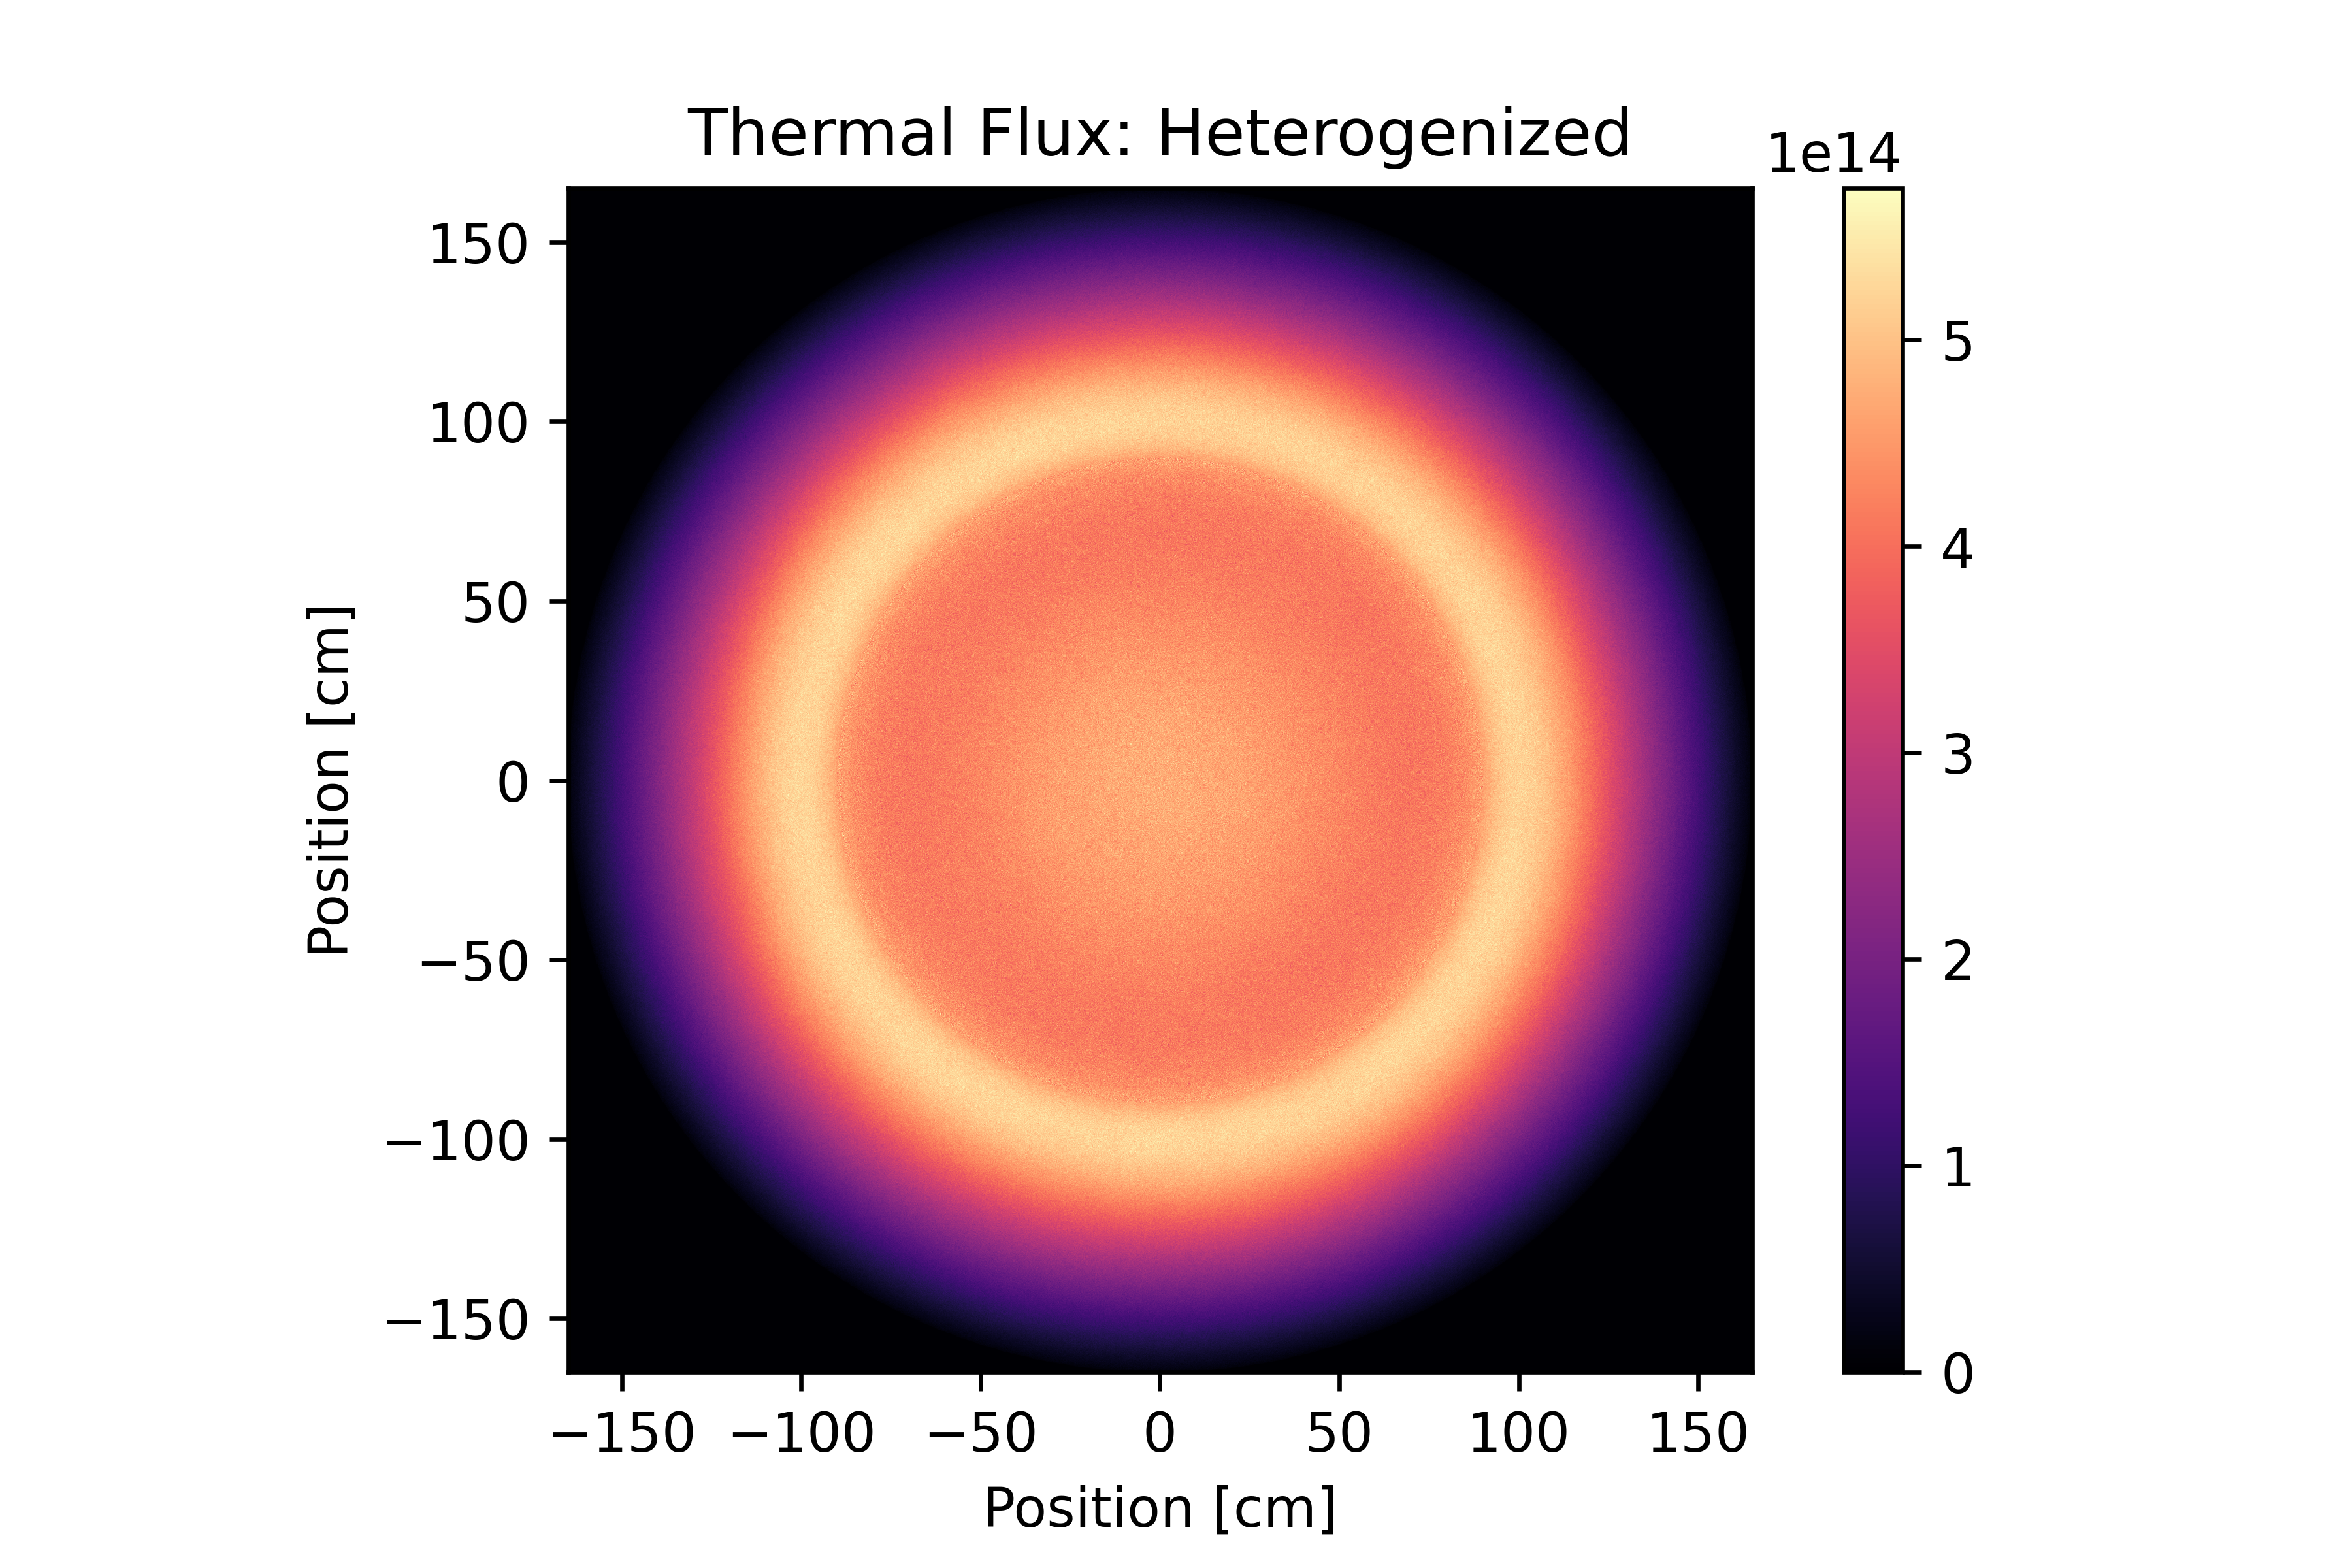
\includegraphics[width=0.95\linewidth]{figures/therm_xy_plane_het.png}
  \caption{Thermal Flux in xy Plane: Heterogenized Pebbles}
  \label{fig:het-plane-therm}
\end{subfigure}%

\begin{subfigure}{0.95\textwidth}
  \includegraphics[width=0.95\linewidth]{figures/fast_xy_plane_het.png}
  \caption{Fast Flux in xy Plane: Heterogenized Pebbles}
  \label{fig:het-plane-fast}
\end{subfigure}

%
\caption{Thermal and Fast Flux Profiles}
\label{fig:het-det-plane}
\end{figure}

Compared with Figure \ref{fig:hom-det-plane}, the edge pebble bands are much less distinct.  This is because the homogenized pebbles have the fissile material spread over the entirety of the 2.5 cm radius fueled center.  The heterogenized pebbles, meanwhile, may have the same number of fissile atoms, but the concentrate the regions capable of fission in the TRISO kernel.  The rest of the pebble consists of its graphite matrix.


\begin{figure}[h!]
\centering
%
\begin{subfigure}{0.25\textwidth}
  \includegraphics[width=0.95\linewidth]{figures/core_spec_het}
  \caption{Core Spectrum}
  \label{fig:het-core}
\end{subfigure}%
%
\begin{subfigure}{0.25\textwidth}
  \includegraphics[width=0.95\linewidth]{figures/fresh_spec_het}
  \caption{Fresh Pebble Spectrum}
  \label{fig:het-fresh}
\end{subfigure}%
%
\begin{subfigure}{0.25\textwidth}
  \includegraphics[width=0.95\linewidth]{figures/6_spec_het}
  \caption{Six-Pass Pebble Spectrum}
  \label{fig:het-six}
\end{subfigure}%

\begin{subfigure}{0.25\textwidth}
  \includegraphics[width=0.95\linewidth]{figures/cool_spec_het}
  \caption{Coolant Spectrum}
  \label{fig:het-cool}
\end{subfigure}%
%
\begin{subfigure}{0.25\textwidth}
  \includegraphics[width=0.95\linewidth]{figures/reflect_spec_het}
  \caption{Reflector Spectrum}
  \label{fig:het-reflec}
\end{subfigure}%
%

\caption{Lethargy Adjusted Neutron Flux Energy Spectra: Core Using Heterogenized Pebbles}
\label{fig:hom-spec}
\end{figure}

The heterogenized spectra, much like the flux profiles, are of a similar morphology.  In order to better examine the differences between the homogenized and heterogenized versions, Figures \ref{fig:diff-flux} and \ref{fig:diff-spec} plot the simple relative difference for all spectra, and the radial fast and thermal profiles.  The relative difference calculation used the following:

\begin{align}
\Delta i &= \frac{i_{hom} - i_{het}}{i_{het}}
\intertext{where}
\Delta i&= \mbox{ relative difference for parameter i between homogenized and heterogenized model }\nonumber\\
i_{hom}&= \mbox{ homogenized parameter i}\nonumber\\
i_{het}&= \mbox{ heterogenized parameter i}\nonumber\\
\end{align}

And error calculation followed simple error propagation rules.


\begin{figure}[h!]
\centering

\begin{subfigure}{0.45\textwidth}
  \includegraphics[width=0.95\linewidth]{figures/reldiff_therm_flux.png}
  \caption{Thermal Flux}
  \label{fig:diff-therm}
\end{subfigure}%
%
\begin{subfigure}{0.45\textwidth}
  \includegraphics[width=0.95\linewidth]{figures/reldiff_fast_flux.png}
  \caption{Fast Flux}
  \label{fig:diff-fast}
\end{subfigure}

%
\caption{Relative Difference in Radial Thermal and Fast Flux Profiles Between Cores Using Homogenized and Heterogenized Pebbles}
\label{fig:diff-flux}
\end{figure}

For both the thermal and flux profiles, error only worsens on the outermost edges.  Overall, Figures \ref{fig:diff-therm} and \ref{fig:diff-fast} suggest that the homogenized simulation is slightly over-predicting the magnitude of the flux; however, given the size of the error, these differences do not exist with certainty.


\begin{figure}[H]
\centering
%
\begin{subfigure}{0.95\textwidth}
  \includegraphics[width=0.95\linewidth]{figures/reldiff_core_spec}
  \caption{Core}
  \label{fig:diff-core}
\end{subfigure}%


\begin{subfigure}{0.95\textwidth}
  \includegraphics[width=0.95\linewidth]{figures/reldiff_fresh_spec}
  \caption{Fresh Pebble}
  \label{fig:diff-fresh}
\end{subfigure}%

\caption{Relative Difference in Lethargy Adjusted Neutron Flux Energy Spectra Between Cores using Homogenized and Heterogenized Pebbles}
\end{figure}

\begin{figure}[H]\ContinuedFloat
\centering

\begin{subfigure}{0.95\textwidth}
  \includegraphics[width=0.95\linewidth]{figures/reldiff_six_spec}
  \caption{Six-Pass Pebble}
  \label{fig:diff-six}
\end{subfigure}%


\begin{subfigure}{0.95\textwidth}
  \includegraphics[width=0.95\linewidth]{figures/reldiff_cool_spec}
  \caption{Coolant}
  \label{fig:diff-cool}
\end{subfigure}%

\caption[]{(cont.)}
\end{figure}

\begin{figure}[H]\ContinuedFloat
\centering

\begin{subfigure}{0.95\textwidth}
  \includegraphics[width=0.95\linewidth]{figures/reldiff_reflec_spec}
  \caption{Reflector}
  \label{fig:diff-reflec}
\end{subfigure}%

\caption[]{(cont.)}
\label{fig:diff-spec}
\end{figure}

Overall, the homogenized model is over-predicting the thermal peak compared with heterogenized in the core spectra by 5\%.  Around $10\times10^{-06}$ MeV, just after the thermal peak, the two spectra agree before diverging again, this time with a slightly greater disagreement.  Unlike Figure \ref{fig:diff-flux}, error alone leaves the relative differences seen in Figure \ref{fig:diff-spec} unaccounted for (with the exception of the highest neutron energy ranges). ***should I leave these, and include an image that gives a close up of the areas of interest, so the huge error at the tail end doesn't keep the reader from seeing detail?***  

The coolant spectra differed after the thermal peak in a magnitude and shape matching the differences in core spectra.  Unlike the core, however, the coolant has much closer agreement at lower energy levels, including at the thermal peak.  The reflector shows a slight over estimation for the homogeneous spectra, which is consistent for all but the highest energy levels.

It is in the pebble spectra that we see the most dramatic disagreement.  Around the thermal peak, in both Figures \ref{fig:diff-fresh} and \ref{fig:diff-six}, the relative difference spikes; though the error is still substantial in this region compared with the peaks in the relative difference.  Between $10\times10^{-07}$ and $5\times10^{-02}$, the differences are minimal and likely accounted for by noise or error.  Between $10\times10^{-02}$ and $10\times10^{-01}$, the difference has a slight blip, which may be indicative of a fission product with a resonance around this region **I don't think I said that quite right***.

The most dramatic peaks occur in the sixth-pass pebble at 0.2995 MeV, at which point the homogenized reactor is over-predicting the lethargy-adjusted neutron flux by a factor of 2.69.  Both the fresh and sixth-pass spectra have another peak at higher energy levels - fresh peaks at 6.3763 MeV, while the sixth-pass spectra has its second peak at 5.2205 MeV.  One possibility is that the $^{235}U$ in the pebble is more likely to undergo fission in a homogenized pebble, which disperses the $^{235}U$ atoms in what is almost pure graphite.



\section{Sensitivity Tests}
Two additional studies look at the effects of assuming a one-sixth core symmetry, and the effects of changing the fuel composition in each pebble, effectively shuffling the pebbles without re-generating their location.  All tests use the homogenized pebble assumption as a base.

\subsection{Effects of Symmetry Assumption}

Overall, the effects of using a one-sixth core symmetry were minimal.



\begin{table}[H]
\centering
 \begin{tabularx}{0.7\textwidth}{c  c  c  c  c}
 	\hline
 	Run & $k_{eff}$ & $k_{eff}$ $\% \Delta$ & $J^+$  $[\frac{n}{cm^2s}]$ & $J^+$ $\% \Delta$  \\
 	\hline
 	Run 1 & 1.01019 $\pm$ 0.00054 & 0.096$\%$ & $7.034\times10^{11}$ $\pm$ $9.988\times10^{08}$ & 0.443$\%$ \\
 	Run 2 & 1.01029 $\pm$ 0.00054 & 0.106$\%$ & $6.979\times10^{11}$ $\pm$ $9.072\times10^{08}$ & 0.347$\%$ \\
 	Run 3 & 1.01116 $\pm$ 0.00057 & 0.192$\%$ & $7.016\times10^{11}$ $\pm$ $1.045\times10^{09}$ & 0.187$\%$ \\
 	Run 4 & 1.00753 $\pm$ 0.00053 & 0.167$\%$ & $7.051\times10^{11}$ $\pm$ $8.320\times10^{08}$ & 0.682$\%$ \\
 	Run 5 & 1.01096 $\pm$ 0.00049 & 0.172$\%$ & $7.000\times10^{11}$ $\pm$ $9.239\times10^{08}$ & 0.046$\%$ \\
 	Run 6 & 1.00997 $\pm$ 0.00056 & 0.074$\%$ & $7.000\times10^{11}$ $\pm$ $1.309\times10^{09}$ & 0.046$\%$ \\
 	\hline

 \end{tabularx}
 \caption[Symmetry Run Results Summary]{Symmetry Run Results Summary.  $\%\Delta$ differences are compared against the control model.}
\label{table:slicesens}
\end{table}

Figure \ref{fig:0-60} provides cross-sections of the geometry, and fission rate/thermal flux meshes for the one-sixth core symmetry test.  The fission rate mesh naturally exhibits a six-part repeating pattern, and still shows the banding patterns on the outer edges. 


\begin{figure}[h!]
\centering

\begin{subfigure}{0.45\textwidth}
  \includegraphics[width=0.95\linewidth]{figures/0-60/0-60-r}
  \caption{Radial Cross Section at y=0}
  \label{fig:0-60-r}
\end{subfigure}%
%
\begin{subfigure}{0.45\textwidth}
  \includegraphics[width=0.95\linewidth]{figures/0-60/0-60-rm}
  \caption{Radial Mesh}
  \label{fig:0-60-rm}
\end{subfigure}

\begin{subfigure}{0.45\textwidth}
  \includegraphics[width=0.95\linewidth]{figures/0-60/0-60-v}
  \caption{Axial Cross Section at z=0 }
  \label{fig:0-60-v}
\end{subfigure}
%
\begin{subfigure}{0.45\textwidth}
  \includegraphics[width=0.95\linewidth]{figures/0-60/0-60-vm}
  \caption{Axial Mesh}
  \label{fig:0-60-vm}
\end{subfigure}
%
\caption{Sensitivity Analysis: $0^{\circ}$ - $60^{\circ}$}
\label{fig:0-60}
\end{figure}
*** alright, I tried to convey my observation as best I could, but I have a suspicion it isn't nearly as clear on paper as it is in my head.  Any suggestions are welcome, and if it seems like it would be better to leave this section out, I can***
One point of interest is the degree to which the region from 0 to 60 degrees matches the same region in the control fission rate mesh.  An image subtraction program generated Figure \ref{fig:htgr-diff} by subtracting the radial meshes for the control (Figure \ref{fig:controlb}) and first symmetry test (Figure \ref{fig:0-60-rm}).

\begin{figure}[h!]
\centering
\includegraphics[width=0.6\linewidth]{figures/htgr-diff}
\caption{An Image Generated by Subtracting \ref{fig:0-60-rm} from \ref{fig:htgr-diff}.}
\label{fig:htgr-diff}
\end{figure}

Within the region between 0 and 60 degrees, the two meshes are almost identical, pixel for pixel.  While this might be unsurprising in the center of this region, the perfect match towards the edges of it are less so.  As a reminder, the symmetry tests all use a one-sixth symmetry, and a periodic boundary condition, i.e., if a neutron leaves the slice on one side, it re-enters the slice on the other.  In effect, the edges of the 0 to 60 degree slice in the symmetry test are seeing entirely different materials, compared with the control.  The edges in \ref{fig:htgr-diff} are not a gradient, but rather a hard line, which may suggest that with proper mixing nearest-neighbor pebbles have a weak effect on core parameters calculated via integration over large portions of the core ***there's 100\% a shorter term for this i'm not thinking of***.  However, note that Sangamon20 uses only fuel pebbles, and this observation may be false in a reactor design using, for example, adsorber pebbles. 


\subsection{Effects of Pebble Shuffling}

The final test on the effects of changes to core modeling is another test of consistency between similar HTGR designs with a different pebble configurations.  Rather than re-generate the pebble locations several times, the 'shuffling' test simply reassigns each pebble with a different fuel composition (creating a new input file).  For example, the pebbles that were once fresh are now first-pass, the first pass pebbles are now second-pass, and so on.  This shuffling happened several times, and the results of this test are in Table \ref{table:shufsens}.



\begin{table}[H]
\centering
 \begin{tabularx}{0.7\textwidth}{c  c  c  c  c}
 	\hline
 	Run & $k_{eff}$ & $k_{eff}$ $\% \Delta$ & $J^+$  $[\frac{n}{cm^2s}]$ & $J^+$ $\% \Delta$ \\
 	\hline
 	Run 1 & 1.03994 $\pm$ 0.00054 & 0.0797$\%$ & $5.897\times10^{11}$ $\pm$ $8.668\times10^{08}$ & 0.626$\%$ \\
 	Run 2 & 1.03999 $\pm$ 0.00055 & 0.0749$\%$ & $5.902\times10^{11}$ $\pm$ $8.086\times10^{08}$  & 0.295$\%$ \\
 	Run 3 & 1.04002 $\pm$ 0.00053 & 0.0721$\%$ & $5.896\times10^{11}$ $\pm$ $8.490\times10^{08}$ & 0.192$\%$  \\
 	Run 4 & 1.04103 $\pm$ 0.00057 & 0.0249$\%$ & $5.884\times10^{11}$ $\pm$ $9.355\times10^{08}$ & 0.013$\%$ \\
 	Run 5 & 1.03960 $\pm$ 0.00053 & 0.112$\%$ & $5.904\times10^{11}$ $\pm$ $8.443\times10^{08}$ & 0.329$\%$  \\
 	Run 6 & 1.04014 $\pm$ 0.00057 & 0.0605$\%$ & $5.898\times10^{11}$ $\pm$ $7.726\times10^{08}$ & 0.227$\%$ \\
 	\hline

 \end{tabularx}
\caption{Shuffling Run Summary}
\label{table:shufsens}
\end{table}

Overall, much like the symmetry test, re-mixing the pebbles had little effect on overall results.  Likely, provided the pebbles are sufficiently mixed, and no 'pockets' of like pebbles exist, designs that are otherwise identical should provide similar results. 